\chapter{Wzorce projektowe}
W latach, kiedy programowanie obiektowe stawało się bardziej popularne, wiele osób natrafiało na grupę problemów pewnej kategorii.
Podczas wielokrotnych prób ich rozwiązywania, różne osoby dochodziły do wspólnych wniosków odnośnie do architektury kodu źródłowego tworzonego w celu ich rozwiązania.
Napotykane wyzwania rozpoczęto dzielić według trzech kategorii: behawioralne, strukturalne oraz kreacyjne. Tak oto to powstały wzorce projektowe.
Obszerna znajomość tej niemałej dziedziny informatyki pozwala spojrzeć na kolejne zadania w znacznie bardziej zaawansowany sposób aniżeli wcześniej.
Można je porównać do znanych przekształceń oraz wzorów matematycznych w rachunku całkowym, gdyż zostały one ściśle zdefiniowane, a osiągniecie efektu końcowego różni się
zastosowanie innych parametrów wejściowych. Podczas tworzenia wzorców usilnie trzymano się zbioru kolejnych zasad znanych pod nazwą SOLID. \newline
Poniżej przedstawiono użyte podczas projektowania sterownika wzorce wraz z fragmentami kodu źródłowego.
\section{Behawioralne}
    \subsection{Komenda}
        Dzięki utworzeniu interfejsu komendy, zrealizowano regułę otwarcia na modyfikacje a zamknięcia na zmiany.
        W przypadku poprawnej definicji funkcjonalności, która powinna zostać zrealizowana, dodajemy jedynie implementację tego interfejsu,
        przez co cała regresja pozostaje bez zmian, a dzięki kontrolerowi, który kolejkuje komendy można pokusić się o realizację kompozytu oraz
        wprowadzenie systemu wag bądź poleceń terminujących aktualnie zaplanowane zadania.
        Podczas implementacji sterownika zastosowano połączenie trzech wzorców projektowych a to wszystko dzięki potężnemu podejściu do organizacji
        struktury kodu jakim jest użycie komend. Zestawiając implementację interfejsu komendy oraz budowania konkretnej wiadomości dzięki fabryce
        pozwala na zdefiniowanie \textit{klas finalnych} zawierających charakterystyczne dla każdej z komend wywołań. 
    \newpage
        \lstinputlisting[
            language=C++,
            caption=Interfejs komendy]
            {Kod_Zrodlowy/DesignPatterns_Command_1.cpp}
        \lstinputlisting[
            language=C++,
            caption=Definicja klasy konkretnej komendy używającej fabryki oraz strategii]
            {Kod_Zrodlowy/DesignPatterns_Command_2.cpp}
        \begin{figure}[h!]
            \centering
            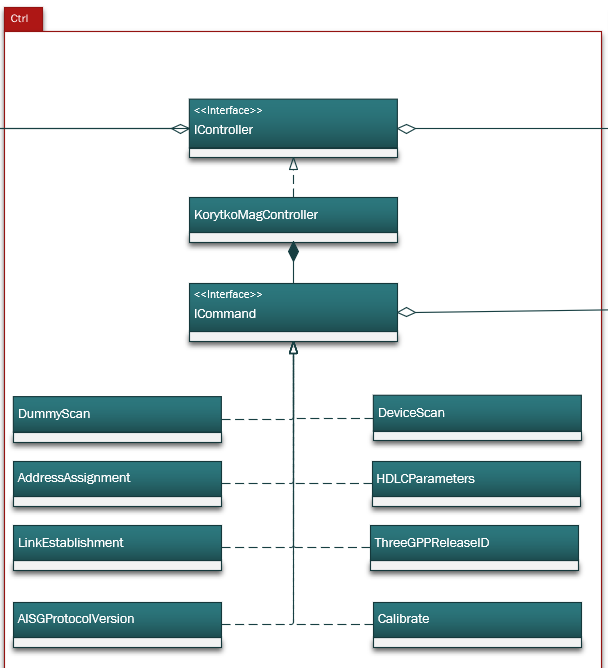
\includegraphics[scale=0.90]{Obrazki/DiagramyKlas/Ctrl.png}
            \caption{Diagram klas przedstawiający realizację wzorca komendy.
                \newline(Opracowanie własne)}
        \end{figure}
    \newpage
    \subsection{Obiekt pusty}
        Znaną przypadłością w językach obiektowych jest wykonywanie dalszej akcji w zależności od stanu pewnego z obiektów.
        W przypadku korzystania ze wskaźników dobrą praktyką jest każdorazowa weryfikacja czy jego wartość nie jest równa \textit{null}.
        Wykorzystanie klasy która implementuje interfejs kontrolera, w sposób neutralny sprawia, że zawsze bezpieczne będzie wywołanie na jej obiekcie 
        instancjonującym którejkolwiek z metod.
    \newpage
        \lstinputlisting[
            language=C++,
            caption=Definicja klasy dla obiektu pustego]
            {Kod_Zrodlowy/DesignPatterns_NullObject_Implementation.cpp}
        \lstinputlisting[
            language=C++,
            caption=Przykład użycia obiektu pustego]
            {Kod_Zrodlowy/DesignPatterns_NullObject_Usage.cpp}
    \newpage
    \subsection{Metoda szablonowa}
        Wprowadzenie systemu walidacji argumentów podanych przez użytkownika gwarantuje bezpieczne wykonywanie akcji niskopoziomowych takich
        jak wysłanie wiadomości do urządzenia, bez zbędnego umieszczanie logiki weryfikacji w dalszym etapie. Zastosowanie tego wzorca umożliwi w przyszłości wdrożenie dodatkowych mechanizmów.
        Jednym z nich jest automatycznie pobranie długiego adresu portu na który ma zostać wysłana komenda, w przypadku podaniu klucza obiektu w bazie danych. 
        Natomiast następnym jest funkcjonalność automatycznej korekty w przypadku zaistniałego błędu syntaktycznego we wprowadzanej przez użytkownika komendzie.
        Obecność komendy ,,execute'' pozwala połączyć wywołanie powyższych funkcji za pomocą jednego polecenia,
        nie posiadając wiedzy o tym jakiego typu procedury weryfikacji sterownik będzie próbował dokonać. Powyższą funkcjonalność osiągnięto dzięki efektownemu wykorzystaniu
        funkcji wirtualnych.
        \lstinputlisting[
            language=C++,
            caption=Plik nagłówkowy dla metody szablonowej walidacji komendy]
            {Kod_Zrodlowy/DesignPatterns_TemplateMethod_Header.hpp}
        \lstinputlisting[
            language=C++,
            caption= Metoda szablonowa - Wywołanie metod wirtualnych z poziomu innej metody]
            {Kod_Zrodlowy/DesignPatterns_TemplateMethod_Implementation.cpp}
    \subsection{Strategia}
        Znanych jest wiele wzorców komunikacji pomiędzy komponentami aczkolwiek w projekcie użyto dwa najbardziej znane: Publikuj-Subskrybuj oraz Żadanie-Odpowiedź.
        
        \begin{figure}[h!]
            \centering
            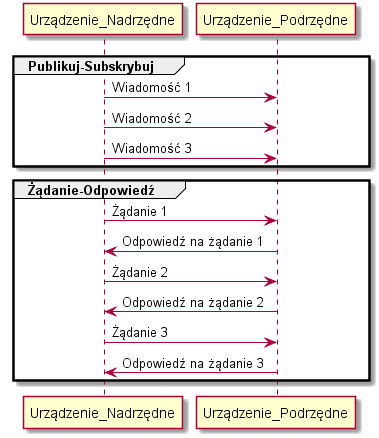
\includegraphics[scale=0.75]{out/Diagramy/PublishSubscribe_RequestResponse.png}
            \caption{Przepływ wiadomości dla wzorca Publikuj-Subskrybuj oraz Żądanie-Odpowiedź.
                \newline(Opracowanie własne)}
        \end{figure}

        Pierwszy z nich efektownie realizuje zasadę odwrócenia zależności, ponieważ sterownik urządzenia nadrzędne na początkowym etapie nie musi znać
        ilości podłączonych do linii urządzeń. Drugi namiast pozwala zrealizować podejście do transmisji z urządzeniem znane jako półdupleks, wymagane podczas
        wywoływania komend zestawiających warstwę łącza danych oraz aplikacyjnej. Głównym problem jest to, że obydwa wzorce wymagają innego zestawu komend w celu
        konfiguracji połączenia ze slotami systemowymi. W projekcie zaimplementowano jeden kontroler, który zarządza zestawianiem wymaganych warstw OSI w trakcie
        ciągłego uruchomienia sterownika, co osiągnięto dzięki dynamicznemu podmianie strategii komunikacji z Publikuj-Subskrybuj na Żadanie-Odpowiedź.
        Zaobserwowano pewne złe następstwo niepoprawnego użycia wzorca strategii polegające na prewencyjnemu rzuceniu wyjątku w przypadku gdyby programista wywołał niepoprawną metode.
        W związku z tym, podczas przyszłej rozbudowy programu, zastosowany zostanie inny wzorzec o nazwie most.
        \newpage
        \lstinputlisting[
        language=C++,
        caption=Strategia komunikacji Żadanie-Odpowiedź dla urządzenia nadrzędnego]
        {Kod_Zrodlowy/DesignPatterns_Strategy.cpp}
    \newpage
    \subsection{Wstrzykiwanie zależności}
        Klasa ,,HDLCCommand'' bezpośrednio dziedziczy po klasie ,,Command''. Dzięki implementacji interfejsu ,,execute'' zrealizowany kontroler posiada możliwość,
        przyszłej rozbudowy nawet o komendy typu ,,włącz muzykę''. W przypadku obsługi urządzenia implementującego protokół AISG, zaobserowowano zapotrzebowanie
        na dodatkową klasę abstrakcyjną, która posiadała będzie wskaźnik na obiekt implementujący interfejs fabryki ramek oraz wzorca komunikacji.
        Podejście programowania sterowanego testami umożliwiło przedstawienie programisty przed koniecznością przekazania powyższych obiektów z poziomu testu, w celu wyeliminowania
        wymagania podłączania fizycznego urządzenia bądź uruchamiania aplikacji symulującej urządzenie oraz skrócenia czasu regresji programu, dzięki
        korzystaniu z atrap.
        Ten sposób zarządzania kolejnością tworzenia oprogramowania naturalnie wymusił realizację wstrzykiwania zależności polegającej na
        przekazywaniu obiektów z zewnątrz podczas wywoływania konstruktora, aniżeli utworzeniu konstruktora zeroparametrowego, 
        który uniemożliwia dalszą modernizacjię elementów składowych systemu.
        \lstinputlisting[
        language=C++,
        caption=Konstruktor zrealizowany podejściem wstrzykiwania zależności]
        {Kod_Zrodlowy/DesignPatterns_DependencyInjection.cpp}
    \subsection{Inicjowanie przy pozyskaniu zasobu}
        Do implementacji pracy użyto kompilator GCC wspierający język C++ w wersji 11-tej, który posiada wbudowany mechanizm inteligentnych wskaźników. ,,shared\_ptr<T>'' oraz ,,unique\_ptr<T>''
        zmieniły sposób korzystania z dynamicznie alokowanej pamięci w sposób diametralny. Do tej pory dealokacja pamięci wskazywanej przez wskaźnik należała do obowiązków programisty.
        Dzięki podejściu tzw. RAII dla ,,shared\_ptr<T>'', w przypadku destrukcji wszystkich wskaźników odnoszących się do wcześniej zaalokowanego obszaru pamięci,
        kompilator przy pomocy destruktora wywołuje komendę ,,delete'' automatycznie, dzięki czemu programista jest ustrzeżony przed niepożądanym wyciekiem pamięci.
\newpage
\section{Kreacyjne}
    \subsection{Budowniczy}
        Często zdarza się, że obiekt klasy wymaga modernizacji wielu z jego pól a realizacja konstruktora posiadającego trzy bądź więcej parametrów,
        uznawana jest za niepoprawną implementacje oraz antywzorzec. W tej sytuacji z pomocą pojawia się wzorzec budowniczego, który podczas wywoływania metody 
        zmieniającej stan obiektu, dokonuje zamierzonego celu, po czym zwraca referencję na obiekt na rzecz którego została wywołana \textit{metoda}. 
        Umożliwia to szeregowe wywoływanie kolejnych modyfikatorów co znacznie oczyściło i zwiększyło czytelność programu. Istnieje wiele interpretacji tego wzorca projektowego,
        w których dodana jest metoda finalizująca budowanie obiektu.
        \lstinputlisting[
            language=C++,
            caption=Budowniczy wraz z Fluent API podczas budowania ramki I - Kalibruj]
            {Kod_Zrodlowy/DesignPatterns_Builder.cpp}
\newpage
    \subsection{Fabryka}
        Istnieje pewien wzorzec, który owiany jest złą sławą. Programiści w momencie usłyszenia o nim dostają ciarek, gdyż sądzą, że pod tym słowem,
        kryje się obiekt, który potrafi zachować się w nieprzewidziany sposób podczas każdorazowego wywoływania jego metod. Z drugiej strony poprawna jego realizacja, 
        umożliwia dynamiczną zmianę wartości zwracanych przed system, a w przypadku sterownika dała możliwość uwspólnienie kodu wraz z symulatorem urządzenia,
        na poziomie 90\%. Mowa o fabryce. W przypadku nieprzechowywania jakiegokolwiek stanu w jej instancji oraz zapoznania się w całości z realizowanym problemem
        komunikacji pomiędzy urządzeniem podrzędnym i nadrzędnym, prawdą jest to, że zaledwie na jedną komendę sterownik nie oczekuje odpowiedzi, a odpowiednie
        nazwanie metod interfejsu fabryki pozwoli zaobserwować, że po obu stronach trzeba obsłużyć komunikację oraz budowę wiadomości charakterystyczną na przykład
        dla polecenia ,,kalibruj'' wprowadzając jedynie niewielkie modyfikacje. 
        \lstinputlisting[
        language=C++,
        caption=Fabryka budowniczych dla sterownika urządzenia nadrzędnego]
        {Kod_Zrodlowy/DesignPatterns_Factory.cpp}
